\documentclass{beamer}
\usepackage[utf8]{inputenc}

\usetheme{Madrid}
\usecolortheme{default}
\usepackage{color}
\usepackage{colortbl}

\usepackage{algorithmic}

\def\HiLi{\leavevmode\rlap{\hbox to \hsize{\color{yellow!50}\leaders\hrule height .8\baselineskip depth .5ex\hfill}}}

\begin{document}

\title{Aprendizagem por Reforço} 
\author{Fabrício Barth}
\institute{Insper Instituto de Ensino e Pesquisa}
\date{Fevereiro de 2024}

\maketitle

\begin{frame}{Contexto}
Até o momento vimos nesta disciplina:
\begin{itemize}
	\item Conceito de Agente Autônomo;
	\item Solução de problemas usando busca em espaço de estados:
	\begin{itemize}
		\item Algoritmos de busca cega, e;
		\item Algoritmos de busca informados.
	\end{itemize}
	\item Busca competitiva.
\end{itemize}
\end{frame}

\begin{frame}{Conteúdo desta aula e das próximas}
  \begin{itemize}
\item Visão Geral sobre Aprendizagem por Reforço
\item Algoritmo \textsc{Q-Learning} e \textsc{Sarsa}
\item Implementações com os projetos \textsc{Gymnasium} e \textsc{PettingZoo}.
%\item Considerações Finais
%\item Material de Consulta
  \end{itemize}
\end{frame}

\begin{frame}{Ao final deste material você saberá}

	\begin{itemize}
	\item o que é \textbf{Aprendizagem por Reforço} e os seus principais conceitos;
	\item como desenvolver um agente autônomo usando os algoritmos \textbf{Q-Learning} e \textbf{Sarsa}, e;
	\item quais os aspectos positivos e negativos dos algoritmos \textbf{Q-Learning} e \textbf{Sarsa}.
	%\item como o algoritmo \textbf{Q-Learning} funciona e como implementá-lo;
	%\item como implementar um \textbf{agente autônomo} usando aprendizagem por reforço, e;
	%\item como implementar um agente autônomo para atuar nos ambientes do \textbf{projeto \textsc{Gym}}.
	\end{itemize}

\end{frame}

\begin{frame}{Taxi Driver - OpenAI Gym}

	\begin{center}
		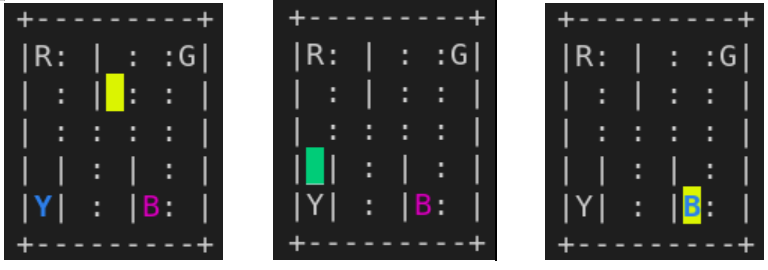
\includegraphics[width=.8\textwidth]{figuras/taxi_driver.png}
	\end{center}

	Podemos implementar uma solução para este problema usando o algoritmo $A^{*}$. Neste caso, 
	\textbf{o que é necessário fazer?}

\end{frame}

\begin{frame}{Taxi Driver - OpenAI Gym}

	Definir uma \textbf{Heurística $H$} que seja admissível e que traga algum valor para o 
	processo de busca.

\end{frame}

\begin{frame}{Ambientes competitivos}

	\begin{center}
		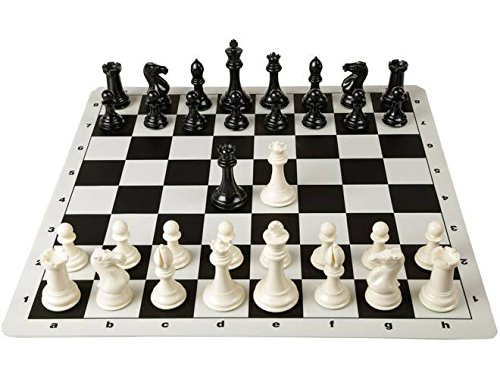
\includegraphics[width=.6\textwidth]{figuras/chess.jpg}
	\end{center}

	Podemos implementar uma solução para este tipo de problema usando o algoritmo 
	\textsc{Min-Max}. Neste caso, \emph{o que é necessário fazer?}

\end{frame}

\begin{frame}{Ambientes competitivos}

	Definir uma \textbf{função de utilidade} que consegue descrever a utilidade dos estados possíveis para o meu agente.


\end{frame}

\begin{frame}{Questão}

	E se fosse possível desenvolver um agente autônomo sem ter que codificar nenhum
	conhecimento sobre a tarefa que ele precisa executar (heurísticas ou funções de utilidade específicas)?

\end{frame}


\begin{frame}{Aprendizagem por Reforço: Visão Geral}
	\small
	Um agente aprende a resolver uma tarefa através de repetidas interações com o ambiente, por tentativa e erro, recebendo 
	(esporadicamente) reforços (punições ou recompensas) como retorno.
  \begin{center}
	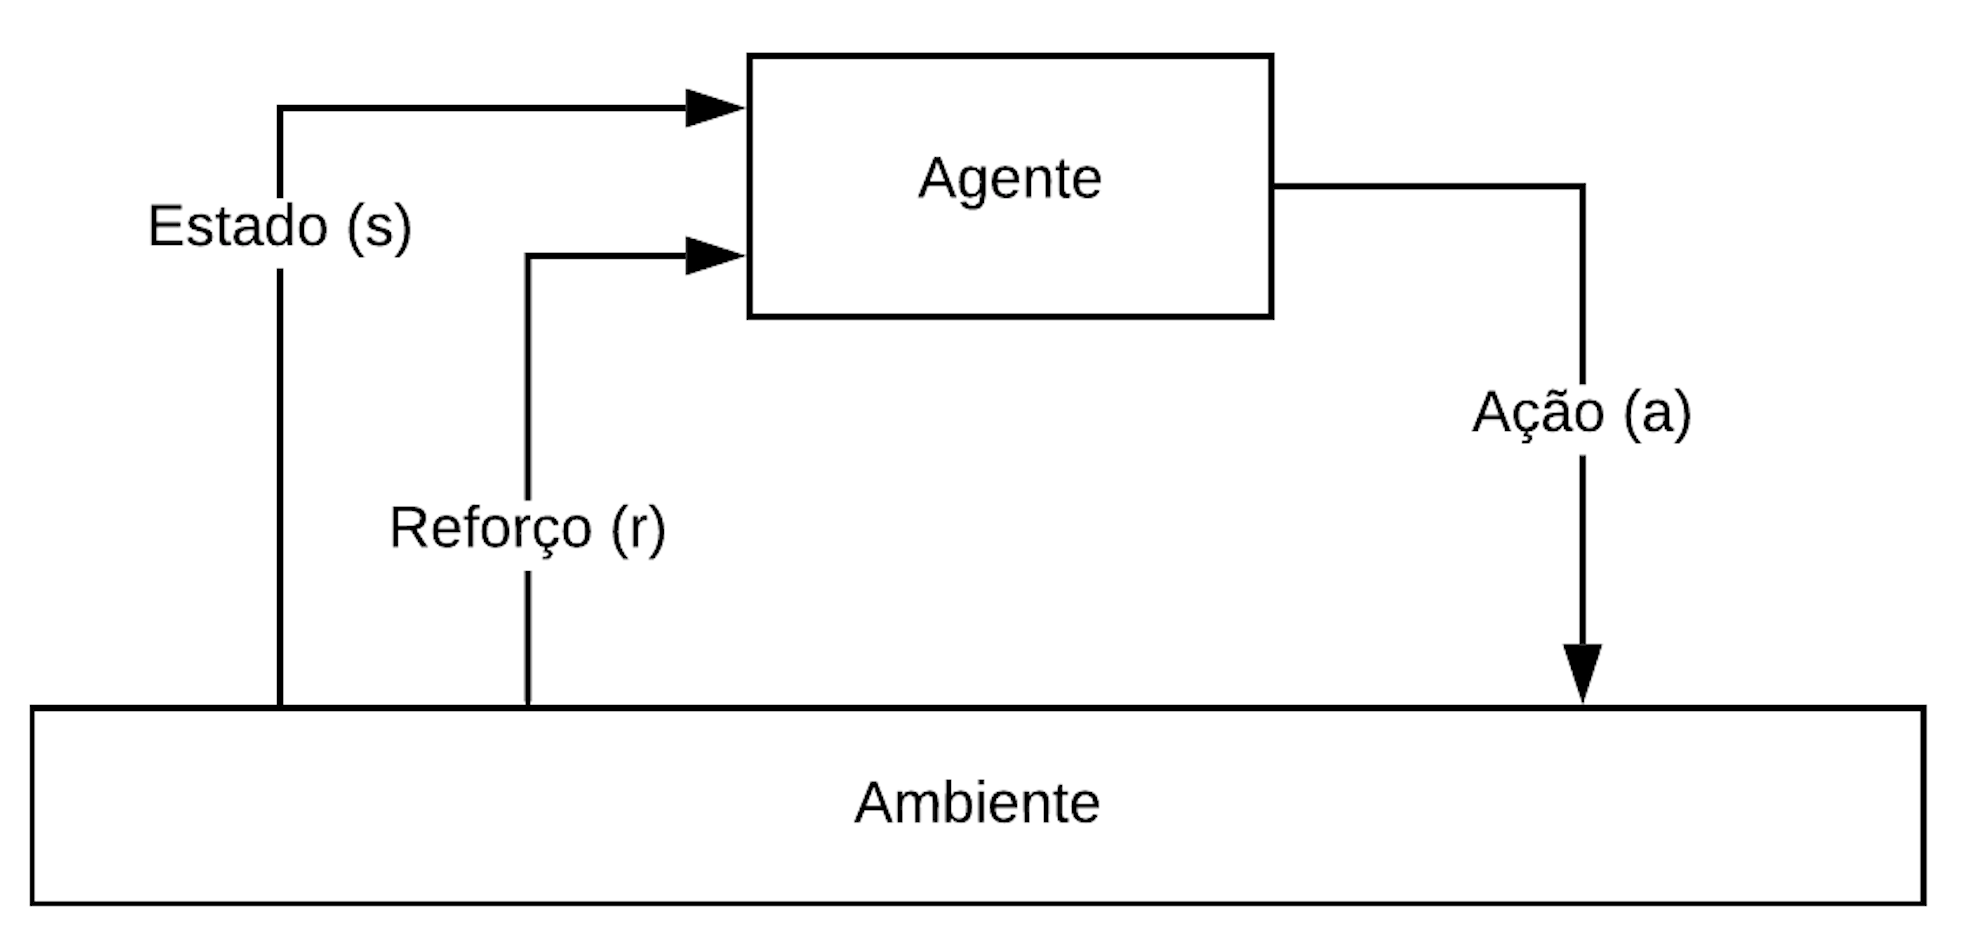
\includegraphics[width=.7\textwidth]{figuras/visaoGeral.png}
\end{center}

\end{frame}

\begin{frame}{Aprendizagem por Reforço: Visão Geral}
	\begin{itemize}
	\item<1-> Este agente não tem conhecimento algum sobre a tarefa que precisa executar (heurísticas ou funções de utilidade específicas).
	\item<2-> Sendo assim, \textbf{{\color{red}como é que o agente consegue atingir um determinado objetivo?}}
	\item<3-> O agente aprende uma \textbf{política de controle}, executando uma \textbf{sequência de ações} por tentativa e erro, e observando as suas \textbf{consequências}.
	
	\end{itemize}
\end{frame}
	



\begin{frame}{Política de Controle}
	\begin{itemize}
	\item A política de controle desejada é aquela que \textbf{maximiza} os reforços 
	(\textit{reward}) acumulados ao longo do tempo pelo 
	agente.
	\item Em tese, é a política que faz o agente percorrer o \textbf{melhor caminho}. 
	\end{itemize}

%\hspace{1cm}

  \begin{center}
	\includegraphics[width=.8\textwidth]{figuras/grafo_rewards_0.png}
\end{center}

\end{frame}


\begin{frame}{Reward acumulado (1/4)}

\begin{center}
	\includegraphics[width=.8\textwidth]{figuras/grafo_rewards_1.png}
\end{center}

\begin{itemize}	
	\item O valor de um estado final leva-se em consideração apenas o 
	reforço: $V(s_{n}) = r_{n}$.
\end{itemize}

\end{frame}


\begin{frame}{Reward acumulado (2/4)}
	
	\begin{center}
		\includegraphics[width=.8\textwidth]{figuras/grafo_rewards_2.png}
	\end{center}
	
	\begin{itemize}	
		\item O $V(s_{2})$ será a soma de $r_{2}$ com o $V(s_{3})$. 
		\item Considerando o fator de desconto $\gamma$, temos: $V(s_{2}) = r_{2} + \gamma^{3} V(s_{3}) $.
		\item O fator de desconto: $0 \leq \gamma < 1$ 
	\end{itemize}
	
\end{frame}

\begin{frame}{Reward acumulado (3/4)}

\begin{center}
	\includegraphics[width=.9\textwidth]{figuras/grafo_rewards_3.png}
\end{center}

\end{frame}

\begin{frame}{Reward acumulado (4/4)}

Desta forma, temos: 

\begin{eqnarray}
V(s_{0}) = r_{0} + \gamma V(s_{1}) \nonumber \\
V(s_{0}) = r_{0} + \gamma r_{1} + \gamma^{2} V(s_{2}) \nonumber \\
V(s_{0}) = r_{0} + \gamma r_{1} + \gamma^{2} r_{2} + \gamma^{3} V(s_{3}) \nonumber \\
V(s_{0}) = r_{0} + \gamma r_{1} + \gamma^{2} r_{2} + \gamma^{3} r_{3} \nonumber
\end{eqnarray}

Ou melhor: 

\begin{equation}
V(s_{0}) = r_{0} + \gamma r_{1} + \gamma^{2} r_{2} + \gamma^{3} r_{3} \cdots + \gamma^{n}r_{n} \nonumber
\end{equation}


\end{frame}


\begin{frame}{Fator de desconto $\gamma$}
	
	\begin{itemize}
		%\item Para tarefas episódicas, o retorno é fácil de ser calculado, 
		%pois será a soma de todas as recompensas obtidas pelo agente. 
		%Mas para tarefas contínuas, como a atividade não tem fim e não podemos 
		%somar até o infinito, há a necessidade da inserção de um fator de 
		%desconto ($\gamma$).
		\item O fator de desconto ($\gamma$) é um hiperparâmetro que consiste 
		em um número entre 0 e 1 que define a importância das recompensas futuras 
		em relação a atual	($0 \leq \gamma < 1$).
		\item Valores mais próximos ao 0 dão mais importância a recompensas 
		imediatas enquanto os mais próximos de 1 tentarão manter a importância 
		de recompensas futuras.
	\end{itemize}
\end{frame}




\begin{frame}{Algoritmo Q-Learning}
	
Para que agente possa identificar uma política de controle ótima este agente 
precisa criar um \textbf{mapeamento} entre \textbf{estados} ($S$) e \textbf{ações} ($A$).

\end{frame}

\begin{frame}{Algoritmo Q-Learning}
	
\begin{itemize}
	
	\item Este mapeamento é representado por uma função $Q(S,A)$ onde $S$ são 
	todos os estados possíveis ($s_{1}, s_{2}, \cdots$) e onde $A$ são todas as 
	ações possíveis ($a_{1}, a_{2}, \cdots$)

\end{itemize}

	\begin{center}
	\begin{tabular}{ |c|c|c|c|c| } 
		\hline
		 \textbf{Q-table}  & $a_{1}$ & $a_{2}$ & $a_{3}$& $a_{4}$ \\
		 \hline
		$s_{1}$&  &  &  & \\ 
		\hline
		$s_{2}$&  &  &  & \\ 
\hline
		$\cdots$&  &  &  & \\ 
\hline
		$s_{n}$&  &  &  & \\ 
\hline
	\end{tabular}
\end{center}

\end{frame}

\begin{frame}{Algoritmo Q-Learning}

	\begin{block}{}
		Como é que o agente pode saber quais são as melhores ações em cada estado?
	\end{block}

\pause

	\begin{itemize}
		\item A ideia é fazer com que o agente aprenda a função de mapeamento $Q(S,A)$. 
		Ou seja, que seja capaz de identificar qual é a melhor ação para cada estado 
		através das suas \textbf{experiências}. 
		\item \textit{Testando} \textbf{infinitas} vezes o ambiente. 
		Ou seja, \textit{testando} \textbf{muitas} vezes as combinações entre 
		\textbf{estados} ($S$) e \textbf{ações} ($A$). 
	\end{itemize}

\end{frame}


\begin{frame}{Algoritmo Q-Learning} 
	\begin{algorithmic} 
		\STATE \emph{\textbf{function} Q-Learning(env, $\gamma$, $\alpha$, episódios)}
		\STATE inicializar os valores de $Q(s, a)$ arbitrariamente
		\FOR {todos os episódios}
		\STATE inicializar $s$ a partir de $env$
		\REPEAT
		\STATE escolher uma ação $a$ para um estado $s$
		\STATE executar a ação $a$
		\STATE observar a recompensa $r$ e o novo estado $s'$ 
		\STATE \HiLi $Q(s,a) \leftarrow Q(s,a) + \alpha[r + \gamma \max_{A'}Q(s',A') - Q(s,a)]$ 
		\STATE$s  \leftarrow s'$
		\UNTIL {$s$ ser um estado final}
		\ENDFOR
		\STATE \textbf{return} $Q(s, a)$
	\end{algorithmic}
\end{frame}

\begin{frame}{Algoritmo Q-Learning: hiperparâmetro $\alpha$}
	\begin{itemize}
		\item $\alpha$ é a taxa de aprendizado ($0 < \alpha \leq 1$), quanto maior, mais valor dá ao novo aprendizado.
	\end{itemize}
\end{frame}

%%\begin{frame}{Algoritmo Q-Learning} 
%%\begin{algorithmic} 
%%	\STATE \textbf{function} Q-Learning(env, $\alpha$, $\gamma$, episódios)
%%	\STATE \emph{inicializar os valores de $Q(s, a)$ arbitrariamente}
%%	\FOR {todos os episódios}
%%	\STATE inicializar $s$ a partir de $env$
%%	\REPEAT
%%	\STATE escolher uma ação $a$ para um estado $s$
%%	\STATE executar a ação $a$
%%	\STATE observar a recompensa $r$ e o novo estado $s'$ 
%%	\STATE $Q(s,a) \leftarrow Q(s,a) + \alpha [r +\gamma \max_{A'}{Q(s', A')} - Q(s,a)]$
%%	\STATE$s  \leftarrow s'$
%%	\UNTIL {$s$ ser um estado final}
%%	\ENDFOR
%%	\STATE \textbf{return} $Q(s, a)$
%%\end{algorithmic}
%
%\end{frame}
%

%\begin{frame}{Algoritmo Q-Learning} 
%\begin{algorithmic} 
%	\STATE \textbf{function} Q-Learning(env, $\alpha$, $\gamma$, episódios)
%	\STATE inicializar os valores de $Q(s, a)$ arbitrariamente
%	\FOR {todos os episódios}
%	\STATE inicializar $s$ a partir de $env$
%	\REPEAT
%	\STATE escolher uma ação $a$ para um estado $s$
%	\STATE executar a ação $a$
%	\STATE observar a recompensa $r$ e o novo estado $s'$ 
%	\STATE \emph{$Q(s,a) \leftarrow Q(s,a) + \alpha [r +\gamma \max_{A'}{Q(s', A')} - Q(s,a)]$}
%	\STATE$s  \leftarrow s'$
%	\UNTIL {$s$ ser um estado final}
%	\ENDFOR
%	\STATE \textbf{return} $Q(s, a)$
%\end{algorithmic}
%
%\end{frame}
%



\begin{frame}{Que ação escolher?} 
	\small
	\begin{algorithmic} 
		\STATE \textbf{function} Q-Learning(env, $\alpha$, $\gamma$, episódios)
		\STATE inicializar os valores de $Q(s, a)$ arbitrariamente
		\FOR {todos os episódios}
		\STATE inicializar $s$ a partir de $env$
		\REPEAT
		\STATE \HiLi \emph{escolher uma ação $a$ para um estado $s$}
		\STATE executar a ação $a$
		\STATE observar a recompensa $r$ e o novo estado $s'$ 
		\STATE $Q(s,a) \leftarrow Q(s,a) + \alpha [r +\gamma \max_{A'}{Q(s', A')} - Q(s,a)]$
		\STATE$s  \leftarrow s'$
		\UNTIL {$s$ ser um estado final}
		\ENDFOR
		\STATE \textbf{return} $Q(s, a)$
	\end{algorithmic}
\end{frame}


\begin{frame}{\textit{Exploration} vs \textit{Exploitation}}
	\begin{itemize}
		\item<1-> A política que o agente utiliza para escolher 
		uma ação $a$ para um estado $s$ não interfere no aprendizado 
		da \textit{Q-table}.
		\item<2-> No entanto, para que o algoritmo \textit{Q-learning} possa convergir 
		para um determinado problema é necessário que o algoritmo visite pares de 
		ação-estado muitas (infinitas) vezes.
		\item<3-> Por isso, que a escolha de determinada \textit{ação} em um \textit{estado} 
		poderia ser feita de forma \textbf{aleatória}. 
		
		\item<4-> Porém, normalmente se utiliza uma política que inicialmente escolhe 
		aleatoriamente as ações, e, à medida que vai aprendendo, passa a utilizar cada 
		vez mais as decisões determinadas pela política derivada de $Q$. 
		
		\item<5-> Esta estratégia inicia \textbf{explorando} (tentar uma ação mesmo que ela não 
		tenha o maior valor de $Q$) e termina escolhendo a ação que tem o 
		maior valor de $Q$ (\textit{exploitation}).  
		
	\end{itemize}
\end{frame}


\begin{frame}{Exemplo de função para escolha de ações}
	
	A escolha de uma ação para um estado é dada pela função:
	
	\vspace{0.3cm}
	
	\begin{algorithmic} 
		\STATE \textbf{function} escolha($s$, $\epsilon$): $a$
		\STATE rv = random ($0 < rv \leq 1$)
		\IF{$rv < \epsilon$}
		\STATE \textbf{return} uma ação $\alpha$ aleatória em $A$
		\ENDIF   
		\STATE \textbf{return} $\max_{a}{Q(s, a)} $
	\end{algorithmic}

	\vspace{0.3cm}
	
	O fator de exploração $\epsilon$ ($0 \leq \epsilon \leq 1$) inicia com um valor 
	alto ($0.7$, por exemplo) e, conforme a simulação avança, 
	diminiu: $\epsilon \leftarrow \epsilon \times \epsilon_{dec}$, 
	onde $\epsilon_{dec} = 0.99$
	
\end{frame}


\begin{frame}{Epsilon}
	  \begin{center}
		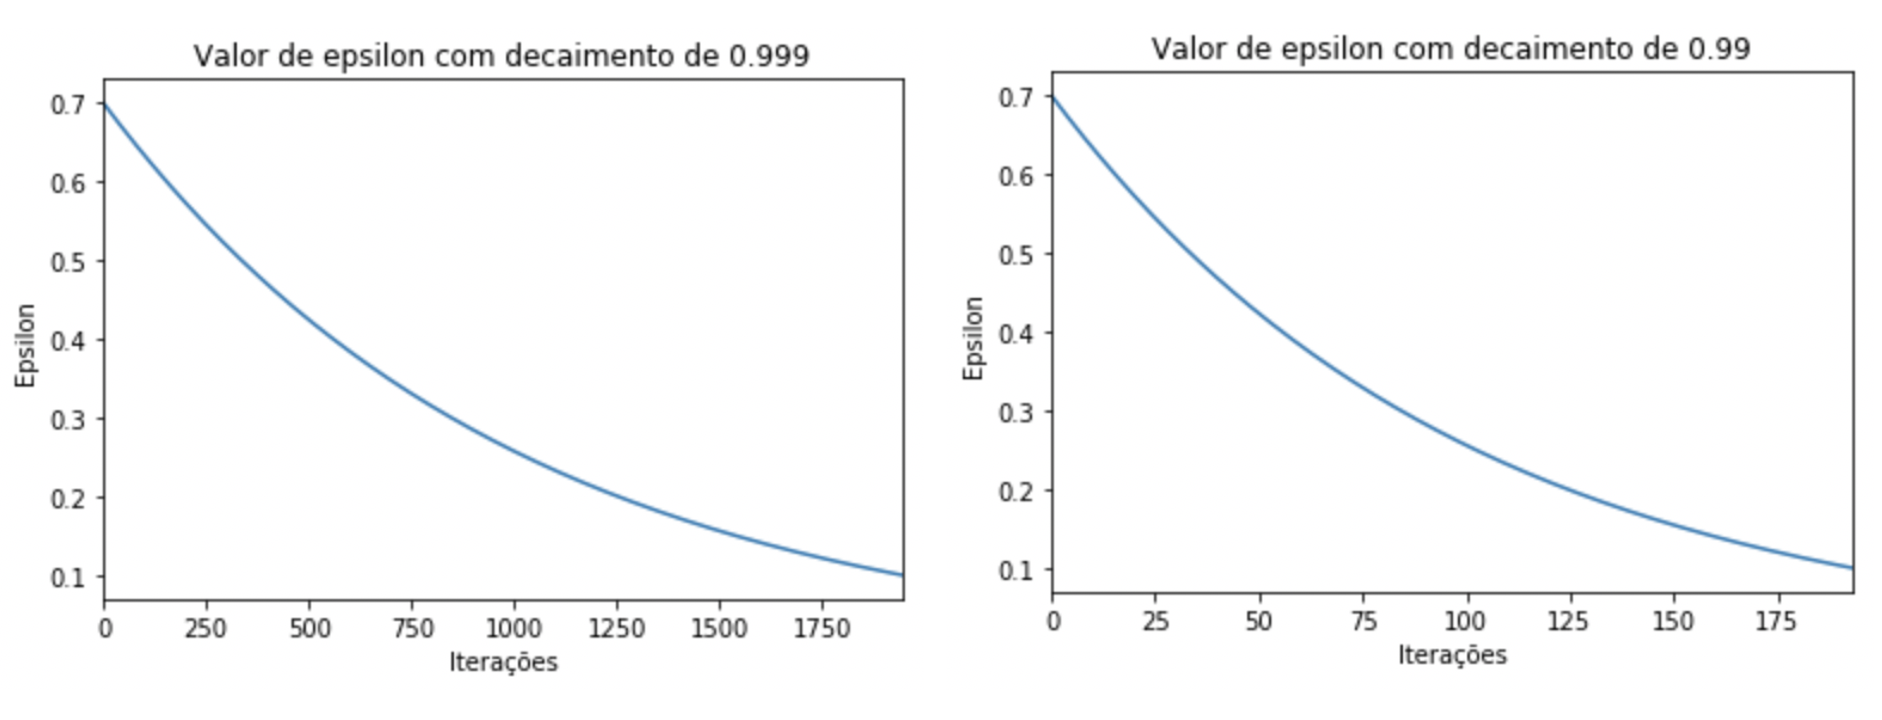
\includegraphics[width=\textwidth]{figuras/epsilon.png}
	\end{center}
\end{frame}

\begin{frame}{Algoritmo Q-Learning}
	
\begin{algorithmic} 
	\STATE \emph{\textbf{function} Q-Learning(env, $\alpha$, $\gamma$, $\epsilon$, $\epsilon_{min}$, $\epsilon_{dec}$, episódios)}
	\STATE inicializar os valores de $Q(s, a)$ arbitrariamente
	\FOR {todos os episódios}
	\STATE inicializar $s$ a partir de $env$
	\REPEAT
	\STATE $a \leftarrow escolha(s, \epsilon)$
	\STATE $s', r \leftarrow$ executar a ação $a$ no $env$
	\STATE $Q(s,a) \leftarrow Q(s,a) + \alpha [r +\gamma \max_{A'}{Q(s', A')} - Q(s,a)]$
	\STATE$s  \leftarrow s'$
	\UNTIL {$s$ ser um estado final}
	\STATE \textbf{if} $\epsilon > \epsilon_{min}$ \textbf{then} $\epsilon \leftarrow \epsilon \times \epsilon_{dec}$
	\ENDFOR
	\STATE \textbf{return} Q
\end{algorithmic}	
\end{frame}

\begin{frame}{Atividade de implementação}
	
	\begin{alertblock}{Atualização da Q-table}
		O objetivo desta atividade é implementar a rotira responsável pela atualização da \textit{Q-table} no arquivo QLearning.py
	\end{alertblock}
	
	\begin{block}{Atividades}
		Siga o roteiro descrito em https://insper.github.io/rl/classes/05\_q\_learning/ \href{https://insper.github.io/rl/classes/05_q_learning/}
		{\beamergotobutton{Link}}
	\end{block}
	
\end{frame}

\begin{frame}{Atividade de implementação}
		
	\begin{alertblock}{Hiperparâmetros e seleção das ações}
		O objetivo desta atividade é compreender o funcionamento e impacto dos hiperparâmetros de $\alpha$, $\gamma$ e dos conceitos de \textit{exploration} e \textit{exploitation}.
	\end{alertblock}
	
	\begin{block}{Atividades}
		Siga o roteiro descrito em https://insper.github.io/rl/classes/05\_x\_hyperparameters/ \href{https://insper.github.io/rl/classes/05_x_hyperparameters/}
		{\beamergotobutton{Link}}
	\end{block}

\end{frame}

\begin{frame}{\textsc{Sarsa}: on-policy}
	
	A regra para update da \textbf{Q-table} no algoritmo \textbf{Q-Learning} é: 
	
	\begin{equation}
	Q(s,a) \leftarrow Q(s,a) + \alpha [r +\gamma \max_{A'}{Q(s', A')} - Q(s,a)]
	\end{equation}

	A diferença entre o novo valor e a estimativa antiga é utilizada para atualizar a estimativa antiga. O algoritmo \textbf{Q-Learning} considera como o novo valor o valor máximo das possibilidades no novo estado $s'$: 
	
	\begin{equation}
	\max_{A'}{Q(s', A')}
	\end{equation}
	
\end{frame}


\begin{frame}{\textsc{Sarsa}: on-policy}
	
	\begin{itemize}
		
	\item No entanto, a ação realmente executada pelo agente pode não ser a ação que tem o valor máximo em $s'$ devido a função de escolha da ação ser baseada no valor de $\epsilon$ e ter características aleatórias.
	
	\item Por isso que o algoritmo \textbf{Q-Learning} é chamado de \textbf{off-policy}.   
\end{itemize}
	
\end{frame}


\begin{frame}{\textsc{Sarsa}: on-policy}
	
	O algoritmo \textsc{Sarsa} é chamado de  \textbf{on-policy} porque ele atualiza a \textbf{Q-table} da seguinte forma: 
	
	\begin{equation}
		Q(s,a) \leftarrow Q(s,a) + \alpha [r +\gamma Q(s', a') - Q(s,a)]
	\end{equation}
	
	o algoritmo \textsc{Sarsa} atualiza $Q(s,a)$ considerando a real ação $a'$ executada pelo agente em $s'$.
	
\end{frame}

\begin{frame}{\textsc{Sarsa}: on-policy}
\begin{algorithmic} 
	\STATE \emph{\textbf{function} Sarsa(env, $\alpha$, $\gamma$, $\epsilon$, $\epsilon_{min}$, $\epsilon_{dec}$, episódios)}
	\STATE inicializar os valores de $Q(s, a)$ arbitrariamente
	\FOR {todos os episódios}
	\STATE inicializar $s$ a partir de $env$
	\STATE \HiLi $a \leftarrow escolha(s, \epsilon)$
	\REPEAT
	\STATE $s', r \leftarrow$ executar a ação $a$ no $env$
	\STATE \HiLi $a' \leftarrow escolha(s', \epsilon)$
	\STATE \HiLi $Q(s,a) \leftarrow Q(s,a) + \alpha [r +\gamma Q(s', a') - Q(s,a)]$
	\STATE $s  \leftarrow s'$
	\STATE \HiLi $a  \leftarrow a'$
	\UNTIL {$s$ ser um estado final}
	\STATE \textbf{if} $\epsilon > \epsilon_{min}$ \textbf{then} $\epsilon \leftarrow \epsilon \times \epsilon_{dec}$
	\ENDFOR
	\STATE \textbf{return} Q
\end{algorithmic}	
\end{frame}


\begin{frame}{Atividade de implementação}
	
	\begin{alertblock}{Comparando \textsc{Q-learning} e \textsc{Sarsa}}
		O objetivo desta atividade é implementar o algoritmo \textsc{Sarsa} e compará-lo com o \textsc{Q-learning}.
	\end{alertblock}
	
	\begin{block}{Atividades}
	Siga o roteiro descrito em https://insper.github.io/rl/classes/05\_x\_sarsa/ \href{https://insper.github.io/rl/classes/05_x_sarsa/}
	{\beamergotobutton{Link}}
	\end{block}

\end{frame} 



%
% ################################ VERSAO 2023 REVISADA ATEH AQUI ########################
%

%\begin{frame}{Ambientes não-determinísticos}
%	
%	\begin{alertblock}{Ambientes não-determinísticos}
%		O objetivo desta atividade é desenvolver agentes capazes de atuar em ambientes não-determinísticos.
%	\end{alertblock}
%	
%	\begin{block}{Atividades}
%		Siga o roteiro descrito em src/parte3/parte3.md \href{https://github.com/fbarth/reinLearn/blob/main/src/parte3/parte3.md}
%		{\beamergotobutton{Link}}
%	\end{block}
%\end{frame}
%
%
%\begin{frame}{Ambiente competitivo com variável aleatória}
%	\begin{alertblock}{Jogos}
%		O objetivo desta atividade é utilizar e analisar o comportamento de agentes em ambientes competitivos com variável aleatória.
%	\end{alertblock}
%	
%	\begin{block}{Atividades}
%		Siga o roteiro descrito em src/parte4/parte4.md \href{https://github.com/fbarth/reinLearn/blob/main/src/parte4/parte4.md}
%		{\beamergotobutton{Link}}
%	\end{block}
%\end{frame}
%
%\begin{frame}{Ambiente contínuo}
%	
%	\begin{alertblock}{Espaço de estados contínuo}
%		O objetivo desta atividade é fazer uso de aprendizagem de reforço em ambientes com um espaço de estados contínuo.
%	\end{alertblock}
%	
%	\begin{block}{Atividades}
%		Siga o roteiro descrito em src/parte5/parte5.md \href{https://github.com/fbarth/reinLearn/blob/main/src/parte5/parte5.md}
%		{\beamergotobutton{Link}}
%	\end{block}
%\end{frame}
%
%
%%%\begin{frame}{Q-Learning com GridSearch}
%%%Faz sentido usar GridSearch para encontrar os melhores valores de $\alpha$ e $\gamma$? 
%%%\end{frame}
%
%
%
%\begin{frame}{Considerações Finais}
%\begin{itemize}
%	\item O algoritmo \textit{Q-Learning} pode ser utilizado por agentes que 
%	não tem conhecimento prévio sobre o problema.
%	
%	%\item Diversos autores já provaram que o algoritmo \textit{Q-Learning} converge 
%	%para a função correta $Q$ dentro de certas condições. Por exemplo, uma 
%	%delas é garantir que o agente avalie um par $Q(s,a)$ diversas vezes.  
%	
%	%\newpage
%	
%	\item \textit{Q-Learning} converge em ambientes 
%	\textbf{determinísticos} e \textbf{não-determinísticos}.
%	
%	\item Na prática, o algoritmo \textit{Q-Learning} necessita de muitas iterações de 
%	treinamento até convergir, inclusive para problemas que não tem um espaço de busca 
%	tão grande.   
%
%\pause 
%
%	\item \textbf{E quando o espaço de busca for muito grande?} 
%
%	%\item Usar \textit{Deep Learning} com \textit{Reinforcement Learning}! \emph{Assunto do 
%	%nosso próximo encontro!}
%
%	%\item Ler o capítulo \textit{18. Reinforcement Learning} até a seção 
%	%\textit{Implementing Deep Q-Learning} do livro \textbf{Hands-On Machine Learning 
%	%with Scikit-Learn, Keras, and TensorFlow, 2nd Edition} do Aurélien Géron.
%
%	%\item Referência adicional: https://deepmind.com/research/case-studies/alphago-the-story-so-far
%
%\end{itemize}
%\end{frame}
%
%
%\begin{frame}{O que vimos até o momento?}
%\begin{itemize}
%	\item o que é \textbf{Aprendizagem por Reforço} e os seus principais conceitos;
%	\item como desenvolver um agente autônomo usando o algoritmo \textbf{Q-Learning};
%	\item quais os aspectos positivos e negativos do algoritmo \textbf{Q-Learning}, e;
%	\item funcionamento da biblioteca \textbf{Gym}. 
%\end{itemize}
%\end{frame}

\begin{frame}{Material de \textbf{consulta}}
\begin{itemize}
  \item Tom Mitchell. Machine Learning. McGraw-Hill, 1997.
  \item Richard S. Sutton and Andrew G. Barto. 2018. Reinforcement Learning: An Introduction. A Bradford Book, Cambridge, MA, USA.
  \item Watkins, C.J.C.H., Dayan, P. Q-Learning. Mach Learn 8, 279–292 (1992). \href{https://doi.org/10.1007/BF00992698}{\beamergotobutton{Link}}
  \item Projeto Gymnasium \href{https://gymnasium.farama.org/}{\beamergotobutton{Link}}
  \item Projeto PettingZoo \href{https://pettingzoo.farama.org/}{\beamergotobutton{Link}}
  %\item https://deepmind.com/research/case-studies/alphago-the-story-so-far
  %\item Aurélien Géron. Hands-On Machine Learning with Scikit-Learn, Keras, and TensorFlow, 2nd Edition, 2019. 
\end{itemize}
\end{frame}

\end{document}

